\begin{auf}
    295
\end{auf}
Bis zu welchem Druck $p_2$ kann der an den Ansaugstutzen (A) einer Wasserstrahlpumpe angeschlossene Rezipient evakuiert werden, wenn der bei 1 in das Strahlrohr vom Durchmesser 13 mm mit Leitungsdruck $p_1=3.2\cdot 10^5Pa$ eintretende Wasserstrahl an der Düse 2 auf den Durchmesser $5mm$ verengt wird, bevor er zusammen mit den aus dem Rezipienten angesaugten Luftmolekülen durch das dahinterliegende Auffangrohr wieder austritt? Der Volumenstrom des Wassers (Dichte $\varrho=10\frac{kg}{m^3}$) beträgt $0.5\frac{l}{s}$.
\begin{figure}[h]
    \centering
    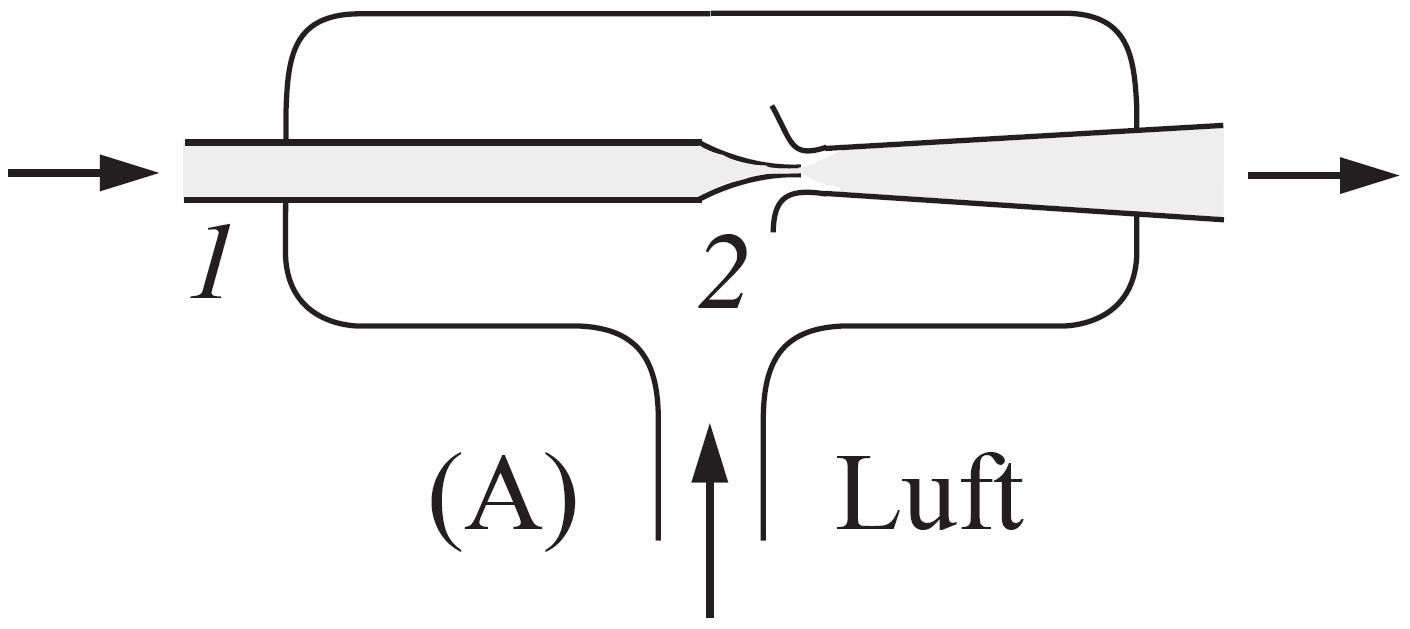
\includegraphics[width=0.7\linewidth]{images/295_0.png}
    \caption{Versuchsaufbau Aufgabe 295}
\end{figure}